\section{UML Models}

\subsection{Use Case Diagram}
	\begin{figure}[h!]
		\centering
		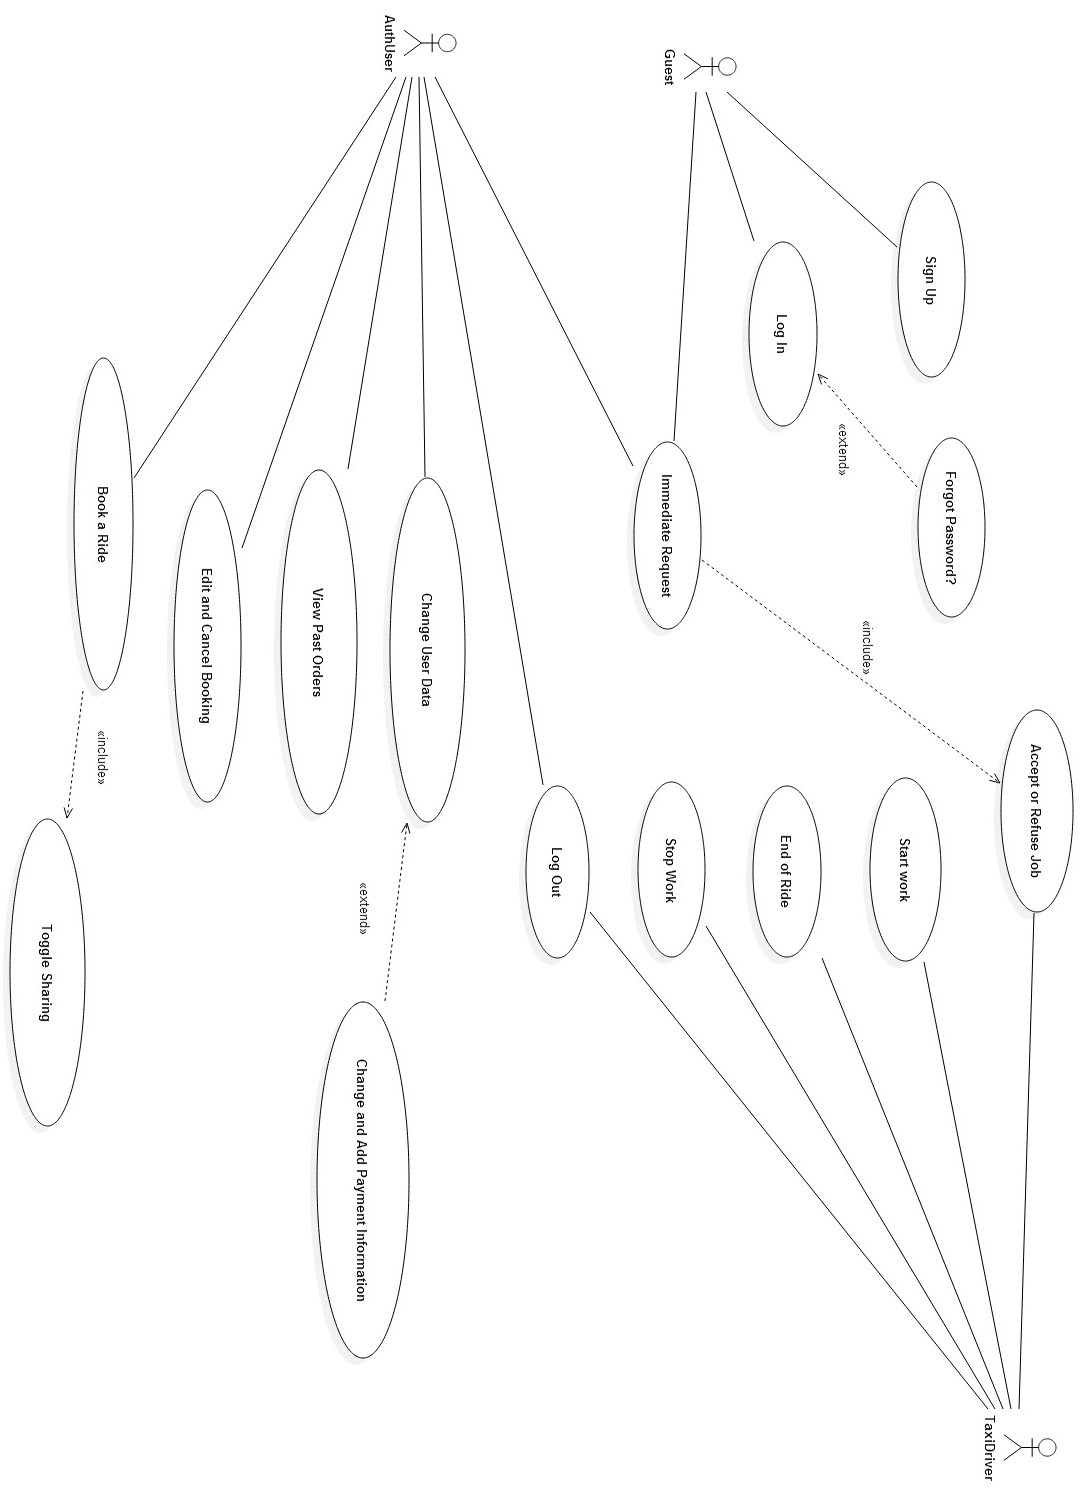
\includegraphics[height=0.85\textheight]{myTaxiServiceImg/UseCase/OverallUseCase.jpg}
	\end{figure}
%\endsubsection
\newpage

\subsection{Use Cases}
These are the use cases which are part of the service
\begin{itemize}
	\item Sign up
	\item Log in
	\item Edit user data
	\item Instant call
	\item Booking ride
	\item Edit booking
	\item Cancel booking
	\item View past rides
	\item Set working condition
	\item Notify end of a ride
	\item Accept or refuse a job
	\item Logout


\end{itemize}


%\endsubsection

\newpage
\subsection{Use Case Description}
These are the detailed descriptions of the Use Cases listed and shown before

\subsubsection{"Sign up" case:}
\hfill \\
\\
\begin {tabular} {|p{3cm}|p{10cm}|}
\hline
Name & Sign up\\
\hline
Actor & Guest\\
\hline
Entry conditions & None\\
\hline
Flow of events &
	\begin {itemize}
		\item The guest enters the website
		\item The guest clicks the SIGN UP button
		\item The guest fills the following fields:
		\begin {itemize}
			\item Name
			\item Surname
			\item E-mail
			\item Date of birth
			\item Password
			\item Payament system $($optional$)$
		\end {itemize}
		\item The Guest clicks on CONFIRM button
	\end {itemize}\\
\hline
Exit conditions & The system shows the home page personalized with the user credential and updates its database.\\
\hline
Exceptions & The guest inserts the wrong email/password combination, the email is already registered in the system or some fields are empthy.\\
\hline
\end {tabular}

\newpage
\subsubsection{"Log in" case:}
\hfill \\
\\
\begin{tabular}{|p{3cm}|p{10cm}|}
\hline
Name & Log in\\
\hline
Actor & Guest\\
\hline
Entry conditions & None\\
\hline
Flow of events & \begin{itemize}
					\item The guest enters the website
					\item The guest fills the text field requested $($email and password$)$
					\item The guest clicks on LOG IN button
				\end{itemize}\\
\hline
Exit conditions & The system shows the home page personalized with the user credential\\
\hline
Exceptions & The guest inserts the wrong email/password combination or the email is not registered in the system\\
\hline
\end {tabular}
\newpage
\begin{figure}[h!]
	\centering
	\includegraphics[height=0.85\textheight]{"myTaxiServiceImg/SequenceDiagram/Log In"}
\end{figure}

\newpage
\subsubsection{"Edit user's data" case:}
\hfill \\
\\
\begin{tabular}{|p{3cm}|p{10cm}|}
\hline
Name & Edit user's data\\
\hline
Actor & User\\
\hline
Entry conditions & None\\
\hline
Flow of events &
	\begin{itemize}
		\item The User clicks on EDIT USER DATA button
		\item The system shows the list of data that the User filled when he signed up
		\item The User modifies the data
		\item The User clicks on SAVE button
		\item The system shows the modified data list
		\item The User click on OK button
	\end{itemize}	\\
\hline
Exit conditions & The system shows the home page personalized with the user credential\\
\hline
Exceptions & The guest inserts wrong new data or doesn't fill all the required fields\\
\hline
\end {tabular}


\newpage
\subsubsection{"Instant call" case:}
\hfill \\
\\
\begin{tabular}{|p{3cm}|p{10cm}|}
\hline
Name & Instant ride\\
\hline
Actor & Guest and User\\
\hline
Entry conditions & None\\
\hline
Flow of events &
	\begin{itemize}
		\item The User either clicks on CALL A TAXI button or HOME button
		\item The system shows the page used to call a taxi
		\item The User chooses if insert an address or use his own position $($via GPS$)$
		\item The User clicks on OK button
	\end{itemize}\\
\hline
Exit conditions & The system shows a confirmation message\\
\hline
Exceptions & None\\
\hline
\end {tabular}

\begin{figure}[h!]
	\centering
	\includegraphics[height=0.4\textheight]{"myTaxiServiceImg/SequenceDiagram/Instant Ride Call"}
\end{figure}


\newpage
\subsubsection{"Book a ride" case:}
\hfill \\
\\
\begin{tabular}{|p{3cm}|p{10cm}|}
\hline
Name & Book a ride\\
\hline
Actor & User\\
\hline
Entry conditions & None\\
\hline
Flow of events &
	\begin{itemize}
		\item The User clicks on BOOK A RIDE button
		\item The system shows a page with the field that the User has to fill:
		\begin{itemize}
			\item Origin position $($can be usd the GPS$)$
			\item Destination
			\item Number of people traveling
			\item Departuring Time
			\item An option to enable the Taxi Sharing
		\end{itemize}
		\item The User fills the fields and clicks OK button or select a similar ride from a pannel and join that ride
	\end{itemize}\\
\hline
Exit conditions & The system shows the confirmation page with the data inserted by the User and updares its booking list\\
\hline
Exceptions & The guest inserts wrong new data like an impossible hour\\
\hline
\end {tabular}

\newpage

\begin{figure}[h!]
	\centering
	\includegraphics[width=0.95\textwidth]{"myTaxiServiceImg/SequenceDiagram/Book a ride"}
\end{figure}


\newpage
\subsubsection{"View status" case:}
\hfill \\
\\
\begin{tabular}{|p{3cm}|p{10cm}|}
\hline
Name & View status\\
\hline
Actor & User\\
\hline
Entry conditions & The User must have booked at least one ride\\
\hline
Flow of events &
	\begin{itemize}
			\item The User clicks on MY BOOKINGS button
			\item The system shows a page with all the User's bookings
			\item The User chooses a shared ride and clicks on STATUS button
			\item The system shows a page with the sharing situation
	\end{itemize}\\
\hline
Exit conditions & The system shows again the User's booking page\\
\hline
Exceptions & None\\
\hline
\end {tabular}

\newpage

\subsubsection{"Edit Booking" case:}
\hfill \\
\\
\begin{tabular}{|p{3cm}|p{10cm}|}
\hline
Name & Edit Booking\\
\hline
Actor & User\\
\hline
Entry conditions & The User must have booked at least one ride\\
\hline
Flow of events &
	\begin{itemize}
			\item The User clicks on MY BOOKINGS button
			\item The system shows a page with all the User's bookings
			\item The User chooses a booking and clicks on STATUS button			
			\item The system shows a page with the reservation's information
			\item The User clicks on MODIFY button
			\item The System shows the page of the booking with the field filled when it was created
			\item The User modifies the data and clicks on SAVE button
	\end{itemize}\\
\hline
Exit conditions & The system shows the confirmation page with the new data of the booking and updates its booking list\\
\hline
Exceptions & The User inserts wrong data like an hour to close to that moment\\
			& The User tries to modify a ride less that ten minutes before its departuring time\\
\hline
\end {tabular}


\newpage
\subsubsection{"Cancel Booking" case:}
\hfill \\
\\
\begin{tabular}{|p{3cm}|p{10cm}|}
\hline
Name & Cancel Booking\\
\hline
Actor & User\\
\hline
Entry conditions & The User must have booked at least one ride\\
\hline
Flow of events &
	\begin{itemize}
		\item The User clicks on MY BOOKINGS button
		\item The system shows a page with all the User's bookings
		\item The User chooses a booking and clicks on STATUS button				
		\item The system shows a page with the reservation's information
		\item The User clicks on CANCEL button
		\item The System shows a page that ask the user to confirm the cancellation
		\item The User clicks the OK button
	\end{itemize}\\
\hline
Exit conditions & The system shows the confirmation page and updates its booking list\\
\hline
Exceptions & The User tries to cancel a booking that has a departure hour that is less than 10 minutes after that moment\\
\hline
\end {tabular}


\newpage

\begin{figure}[h!]
	\centering
	\includegraphics[height=0.95\textheight]{"myTaxiServiceImg/SequenceDiagram/Edit or cancel a booking"}
\end{figure}


\newpage
\subsubsection{"View past rides" case:}
\hfill \\
\\
\begin{tabular}{|p{3cm}|p{10cm}|}
\hline
Name & View past rides\\
\hline
Actor & User\\
\hline
Entry conditions & The User must have ordered at least one ride\\
\hline
Flow of events &
	\begin{itemize}
		\item The User clicks on MY BOOKINGS button
		\item The system shows a page with all the User's bookings $($if there are any$)$ and the booking history
		\item The User can see the details of a particular booking by selecting one
	\end{itemize}\\

\hline
Exit conditions & The system shows again the User's booking page\\
\hline
Exceptions & None\\
\hline
\end {tabular}

\newpage
\subsubsection{"Set Working Condition" case:}
\hfill \\
\\
\begin {tabular}{|p{3cm}|p{10cm}|}
\hline
Name & Set Working Condition\\
\hline
Actor & Taxi Driver\\
\hline
Entry conditions & None\\
\hline
Flow of events &
	\begin {itemize}
		\item The Driver clicks on MODIFY WORKING STATE button
		\item The system shows a page with the current working state and, if the state is on "working", the amount of time the Driver has been working
		\item The Driver clicks on SET WORKING or SET NOT WORKING button to set his situation
		\item The system shows the working state page updated
	\end {itemize}\\

\hline
Exit conditions & The system updates the Driver's condition\\
\hline
Exceptions & None\\
\hline
\end {tabular}


\newpage

\subsubsection{"Accept or refuse a job" case:}
\hfill \\
\\
\begin {tabular}{|p{3cm}|p{10cm}|}
\hline
Name & Accept or refuse a job\\
\hline
Actor & Taxi Driver\\
\hline
Entry conditions & The Driver must have been notified of the presence of a possibile ride\\
\hline
Flow of events &
	\begin {itemize}
		\item The Driver opens the notification
		\item The system shows a page the data of the ride
		\item The Driver clicks on ACCEPT or REFUSE button
		\item The system shows a confirmation page
	\end {itemize}\\
\hline
Exit conditions & The system either notifies the asker and removes the Driver from the queue if he accepted, or moves the Driver to the bottom of the queue if he refused\\
\hline
Exceptions & None\\
\hline
\end {tabular}


\newpage
\begin{figure}[h!]
	\centering
	\includegraphics[height=0.95\textheight]{"myTaxiServiceImg/SequenceDiagram/Edit or cancel a booking"}
\end{figure}
\newpage

\subsubsection{"Notify the end of a ride" case:}
\hfill \\
\\
\begin {tabular}{|p{3cm}|p{10cm}|}
\hline
Name & Notify the end of a ride\\
\hline
Actor & Taxi Driver\\
\hline
Entry conditions & The Driver must have already accepted a ride\\
\hline
Flow of events &
	\begin{itemize}
		\item The Driver clicks on the RIDE COMPLETED button in his homepage
		\item The system shows a page to ask for confirmation
		\item The Driver clicks on the OK or CANCEL button to confirm or not
		\item The system shows the homepage again
	\end{itemize}\\

\hline
Exit conditions & The system add the Driver to the queue\\
\hline
Exceptions & None\\
\hline
\end {tabular}
\\
\\
\\
\\
\\

\subsubsection{"Log Out" case:}
\hfill \\
\\
\begin {tabular}{|p{3cm}|p{10cm}|}
\hline
Name & Log Out\\
\hline
Actor & User and Taxi Driver\\
\hline
Entry conditions & None\\
\hline
Flow of events &
	\begin{itemize}
		\item The user clicks on LOG OUT button
		\item The system shows the Guest's homepage
	\end{itemize}\\
\hline
Exit conditions & None\\
\hline
Exceptions & None\\
\hline
\end {tabular}



%\endsubsection

\subsection{State Charts}


\subsubsection{Reservation}

This statechart describes the status of a reservation from creation to completion

	\begin{figure}[h!]
		\centering
		\includegraphics[height=0.75\textheight]{"myTaxiServiceImg/SequenceDiagram/Booking"}
	\end{figure}

\newpage
\subsubsection{Driver Status}

This statechart follows the status of a Taxi Driver throughout the workday

	\begin{figure}[h!]
		\centering
		\includegraphics[height=0.85\textheight]{"myTaxiServiceImg/SequenceDiagram/Driver Status"}
	\end{figure}

\newpage
\subsection{UML Class Diagram}
	\begin{figure}[h!]
		\centering
		\includegraphics[height=0.75\textheight]{"myTaxiServiceImg/SequenceDiagram/myTaxiServiceUMLjpeg"}
	\end{figure}
%\endsubsection